\documentclass[12pt,a4paper]{article}

\usepackage[brazil]{babel}
\usepackage{fontspec}
\usepackage{xeCJK}
\usepackage{xcolor}
\usepackage{ruby}
\usepackage{amsmath}
\usepackage{tcolorbox}
\usepackage{enumitem}
\usepackage{tabularx}
\usepackage{booktabs}

\setmainfont{Latin Modern Roman}
\setCJKmainfont{Noto Serif CJK JP}

\definecolor{jpnavy}{RGB}{20, 35, 60}
\definecolor{jpred}{RGB}{180, 40, 40}
\definecolor{lighthight}{RGB}{245, 247, 250}
\definecolor{jppurple}{RGB}{110, 70, 120}

\pagestyle{empty}

\begin{document}

\begin{center}
    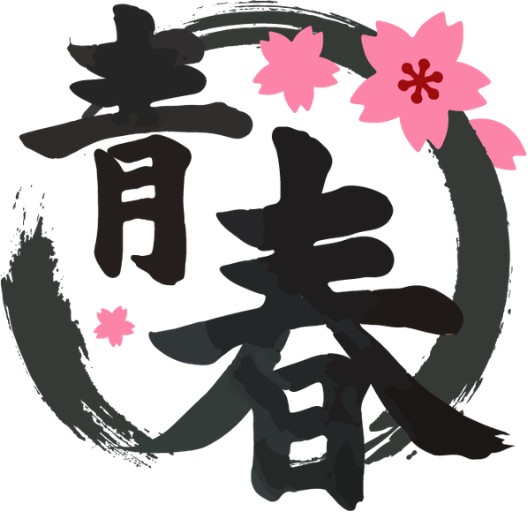
\includegraphics[height=2cm, keepaspectratio]{../Seishun.png}\\
    \vspace{0.3cm}
    {\LARGE\bfseries 第八課}\\[4pt]
    \small Família e Relações
\end{center}

\vspace{0.3cm}
\hrule height 1pt
\vspace{0.5cm}

\begin{tcolorbox}[colback=jppurple!6, colframe=jppurple, title=\textbf{Dica Cultural \& Linguagem de Tratamento}, fonttitle=\bfseries]
\small
Em japonês, a forma como nos referimos à nossa própria família (visão de humildade / \textit{Uchi}) é diferente da forma como nos referimos à família dos outros (visão de respeito / \textit{Soto}). Por exemplo: minha mãe é \textbf{Haha}, mas a mãe de outra pessoa é \textbf{Okaasan}.
\end{tcolorbox}

\vspace{0.2cm}

\subsection*{Árvore Genealógica e Relações (\textit{Kazoku no Yobikata})}

\vspace{0.2cm}

\noindent
\small
\begin{tabularx}{\textwidth}{>{\bfseries\color{jpnavy}}l X X}
\toprule
Grau de Parentesco & Minha Família (\textit{Uchi}) & Família de Outro (\textit{Soto}) \\
\midrule
Avô & 祖父 (\textit{Sofu}) & おじいさん (\textit{Ojiisan}) \\
Avó & 祖母 (\textit{Sobo}) & おばあさん (\textit{Obaasan}) \\
Pai & 父 (\textit{Chichi}) & おとうさん (\textit{Otousan}) \\
Mãe & 母 (\textit{Haha}) & おかあさん (\textit{Okaasan}) \\
Irmão Mais Velho & 兄 (\textit{Ani}) & おにいさん (\textit{Oniisan}) \\
Irmã Mais Velha & 姉 (\textit{Ane}) & おねえさん (\textit{Oneesan}) \\
Irmão Mais Novo & 弟 (\textit{Otouto}) & 弟さん (\textit{Otouto-san}) \\
Irmã Mais Nova & 妹 (\textit{Imouto}) & 妹さん (\textit{Imouto-san}) \\
Esposo(a) / Cônjuge & 夫 / 妻 (\textit{Otto / Tsuma}) & ご主人 / 奥さん (\textit{Goshujin / Okusan}) \\
Filho(a) & 息子 / 娘 (\textit{Musuko / Musume}) & 息子さん / 娘さん (\textit{-san}) \\
\bottomrule
\end{tabularx}

\vspace{0.3cm}

\noindent
\small
\begin{tabularx}{\textwidth}{>{\bfseries\color{jpnavy}}l X X}
\toprule
\multicolumn{3}{c}{\textbf{\color{jpnavy}Grupos, Plurais e Amigos (Sufixo ～たち - \textit{-tachi})}} \\
\midrule
Nós / Nosso grupo & 私たち (\textit{Watashitachi}) & Refere-se a "nós" / meu grupo. \\
Amigos / Meus amigos & 友達 (\textit{Tomodachi}) / 友達たち & Círculo de amizades. \\
Crianças / Filhos & 子供たち (\textit{Kodomotachi}) & Grupo de crianças ou filhos. \\
\bottomrule
\end{tabularx}

\newpage

\begin{center}
    {\LARGE\bfseries 会話 (Diálogo em Família)}
\end{center}

\textit{Cenário: Em casa, no final da tarde, a mãe (Okaasan) conversa com o filho (Ren) e o irmão mais velho (Onii-chan) sobre o jantar e as tarefas domésticas.}

\vspace{0.8em}

\textbf{\ruby{母}{おかあさん}:} 蓮、お兄ちゃん、もうすぐ晩ご飯の時間だよ！手伝ってくれる？\\
\textit{Okaasan:} Ren, Onii-chan, mousugu ban-gohan no jikan da yo! Tetsudatte kureru?\\
Mãe: Ren, filho mais velho, já é quase hora do jantar! Podem me ajudar?

\vspace{0.4em}

\textbf{\ruby{蓮}{れん}:} はーい！お母さん、今日の夜ご飯は何？\\
\textit{Ren:} Haai! Okaasan, kyou no yoru-gohan wa nan?\\
Ren: Siiiim! Mãe, o que é o jantar de hoje?

\vspace{0.4em}

\textbf{\ruby{母}{おかあさん}:} 今夜はカレーだよ。蓮はテーブルを拭いて、お皿を並べてね。\\
\textit{Okaasan:} Kon'ya wa karē da yo. Ren wa tēburu wo fuite, o-sara wo narabete ne.\\
Mãe: Hoje à noite é curry. Ren, limpe a mesa e organize os pratos, tá bom?

\vspace{0.4em}

\textbf{\ruby{お兄ちゃん}{おにいちゃん}:} じゃあ、僕がお米を研いで、ご飯を炊くよ！\\
\textit{Onii-chan:} Jaa, boku ga o-kome wo toide, gohan wo taku yo!\\
Irmão Mais Velho: Então eu vou lavar o arroz e colocar para cozinhar!

\vspace{0.4em}

\textbf{\ruby{母}{おかあさん}:} ありがとう！食べた後は、みんなで皿洗いをしましょうね。\\
\textit{Okaasan:} Arigatou! Tabeta ato wa, minna de sara-arai wo shimashou ne.\\
Mãe: Obrigada! Depois de comer, vamos lavar a louça juntos.

\vspace{0.4em}

\textbf{\ruby{蓮}{れん}:} うん！ご飯の後は僕が掃除もするよ。\\
\textit{Ren:} Un! Gohan no ato wa boku ga souji mo suru yo.\\
Ren: Sim! Depois do jantar eu também faço a limpeza.

\newpage

\subsection*{Vocabulário Útil: Tarefas Domésticas e Rotina (\textit{Tango})}

\vspace{0.2cm}

\noindent
\small
\begin{tabularx}{\textwidth}{>{\bfseries\color{jpnavy}}l X X}
\toprule
Palavra (Romaji) & Kanji / Kana & Tradução em Português \\
\midrule
Kaji & 家事 (かじ) & Tarefas domésticas / Afazeres do lar \\
Ban-gohan / Yoru-gohan & 晩ご飯 / 夜ご飯 & Jantar / Refeição da noite \\
Sara-arai & 皿洗い (さらあらい) & Lavar a louça \\
Souji & 掃除 (そうじ) & Limpeza (da casa) \\
Sentaku & 洗濯 (せんたく) & Lavar roupa \\
Ryouri & 料理 (りょうり) & Cozinhar / Preparar a comida \\
\midrule
Kokuban / Kurosuto & 黒板 (こくばん) & Lousa / Quadro-negro \\
Tēburu wo fuku & テーブルを拭く & Limpar / Passar pano na mesa \\
Gohan wo taku & ご飯を炊く & Cozinhar arroz \\
Tetsudau & 手伝う (てつだう) & Ajudar / Auxiliar \\
\bottomrule
\end{tabularx}

\vspace{0.5cm}

\begin{tcolorbox}[colback=jppurple!6, colframe=jppurple, title=\textbf{Dinâmica em Grupo (Prática Presencial)}, fonttitle=\bfseries]
\small
Descubra como vai a família do seu colega e se ele(a) tem irmãos!

\vspace{0.2cm}

\begin{enumerate}[leftmargin=*]
    \item \textbf{Perguntar sobre irmãos:} \textit{Kyoudai ga imasu ka?} (Você tem irmãos?)
    \item \textbf{Responder com a quantidade de irmãos:} \textit{Hai, [Número + nin] imasu.} (Ex: \textit{Hai, ani ga hitori to imouto ga hitori imasu}) ou \textit{Ie, hitorikko desu} (Não, sou filho único).
    \item \textbf{Perguntar sobre a família:} \textit{Go-kazoku wa genki desu ka?} (Como vai a sua família?)
\end{enumerate}
\end{tcolorbox}

\vspace{0.4cm}

\begin{center}
    \small\color{gray} \textit{お疲れ様でした！}
\end{center}

\end{document}
